\documentclass[]{article}
\usepackage{amsmath}
\usepackage{fancyhdr}
\linespread{1.5}
\usepackage{subcaption}
\usepackage{tikz-qtree}
\usepackage{mathtools}
\usepackage[headsep=1cm, top=1.58cm,bottom=1cm,right=1.5cm,left=1.5cm]{geometry}
\usepackage[utf8]{inputenc}
\usepackage{lmodern, textcomp}
\usetikzlibrary{shapes,arrows.meta,positioning,bending}
\tikzset{every tree node/.style={minimum width=2em,draw,circle},
     blank/.style={draw=none},
     edge from parent/.style=
     {draw, edge from parent path={(\tikzparentnode) -- (\tikzchildnode)}},
     level distance=1.5cm}



\tikzstyle{process} = [rectangle,rounded corners,minimum width=3cm, minimum height=1cm, text centered, draw=black, fill=orange!15]

\tikzstyle{decision} = [diamond,aspect=2, minimum width=3cm, minimum height=1cm, text centered, draw=black, fill=pink]

\tikzstyle{arrow} = [thick,->,>=stealth]
\pagestyle{fancy}
\fancyhf{}
\usepackage{graphicx}
\usepackage{hyperref}
\usepackage{xepersian}
\settextfont{Yas}
\author{پارسا پورسیستانی-۹۹۱۳۰۳۶}

\newcommand{\gu}[1]{«#1»}
\headheight 75pt
\begin{document}
\begin{titlepage}
\newcommand{\HRule}{\rule{\linewidth}{0.5mm}} 
\newcommand{\itab}[1]{\hspace{0em}\rlap{#1}}

\center 

\includegraphics[scale=0.15]{logo2.png}\\[1cm]
\textsc{\LARGE \bfseries دانشکده ریاضی و علوم‌کامپیوتر}\\[0.7cm] 
\textsc{\Large \bfseries عنوان تمرین}\\[0.5cm] 
\HRule \\[0.4cm]
{ \huge \bfseries اسم درس}\\[0.4cm]
\HRule \\[1cm]
\textsc{\LARGE \bfseries پارسا پورسیستانی-۹۹۱۳۰۳۶}\\[0.7cm]
\end{titlepage}
\newpage
\rhead{
	\includegraphics[height=25mm]{logo.png}
	}
\lhead{
	\textsc{\large \bfseries  عنوان تمرین}
}
\chead{
	\textsc{\large \bfseries  اسم درس}
}
  
\section*{سوال ۱.}

لورم ایپسوم متن ساختگی با تولید سادگی نامفهوم از صنعت چاپ، و با استفاده از طراحان گرافیک است، چاپگرها و متون بلکه روزنامه و مجله در ستون و سطرآنچنان که لازم است، و برای شرایط فعلی تکنولوژی مورد نیاز، و کاربردهای متنوع با هدف بهبود ابزارهای کاربردی می باشد، کتابهای زیادی در شصت و سه درصد گذشته حال و آینده، شناخت فراوان جامعه و متخصصان را می طلبد، تا با نرم افزارها شناخت بیشتری را برای طراحان رایانه ای علی الخصوص طراحان خلاقی، و فرهنگ پیشرو در زبان فارسی ایجاد کرد، در این صورت می توان امید داشت که تمام و دشواری موجود در ارائه راهکارها، و شرایط سخت تایپ به پایان رسد و زمان مورد نیاز شامل حروفچینی دستاوردهای اصلی، و جوابگوی سوالات پیوسته اهل دنیای موجود طراحی اساسا مورد استفاده قرار گیرد.
  \begin{center}
    \begin{tabular}{|c|c|c|}
    \hline
         نام & پارسا & پورسیستانی \\
    \hline

رشته &
\multicolumn{2}{|c|}{علوم‌کامپیوتر}
\\
\hline
         شغل & دانشجو & کارشناسی \\
    \hline 
    
    شماره‌دانشجویی &
\multicolumn{2}{|c|}{۹۹۱۳۰۳۶}
\\
\hline
    
    \end{tabular}
  \end{center}
\begin{center}
\end{center}
\newpage
\section*{سوال ۲.}
Each of the exercises below involves a choice among the master theorem templates discussed in lecture.
For each, indicate which case applies and specify the asymptotic growth class of the function.  If no
case applies, simply state that fact; you are not required to attempt a solution when no master theorem case
applies.

\begin{enumerate}
\item $T(n) = 2 T(\lfloor n/4 \rfloor) + n^{1/2}$.
\item $T(n) = 3 T(\lfloor n/2 \rfloor) + n \lg n$.
\item $T(n) = 5 T(\lfloor n/5 \rfloor) + \frac{n}{\lg n}$.
\item $T(n) = 4 T(\lfloor n/2 \rfloor) + n^2 \sqrt{n}$.
\item $T(n) = 2 T(\lfloor n/2 \rfloor) + n \lg n$.
\end{enumerate}

\section*{Solutions.}
$a = 3, b = 2$ implies a reference function $g(n) = n^{\log_2 3}$. Converting as follows,
\begin{eqnarray*}
y & = & \log_2 3 \\
2^y & = & 3 \\
y \ln 2 & = & \ln 3 \\
y & = & \frac{\ln 3}{\ln 2} = 1.585,
\end{eqnarray*}
we have $g(n) = n^{1.585}$.  The ``glue'' function is $f(n) = n \lg n$.  Let $g_\epsilon (n) = n^{1.585 - \epsilon}$, for 
$0 < \epsilon < 0.5$. Since
\begin{eqnarray*}
\frac{f(n)}{g_\epsilon (n)} & = & \frac{n \lg n}{n^{1.585 - \epsilon}} = \frac{\lg n}{n^{0.585 - \epsilon}} \\
 & \leq & \frac{\lg n}{n^{0.085}} \rightarrow 0
\end{eqnarray*}
as $n \rightarrow \infty$, we have $f(n) = o(g_\epsilon (n))$, which implies $f(n) = O(g_\epsilon (n))$ and allows case (1) of the 
master template.  Therefore $T(n) = \Theta(g(n)) = \Theta(n^{1.585})$.
\newpage

\section*{سوال ۳.}
\begin{figure}[!ht]
\centering
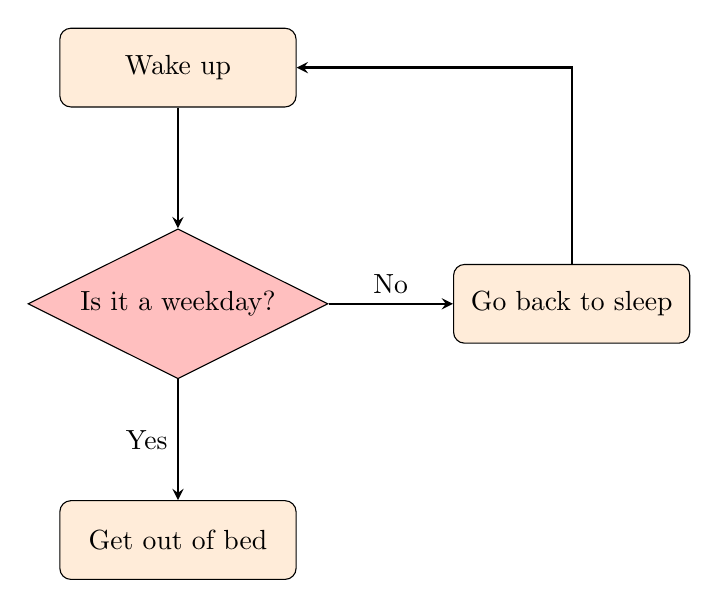
\begin{tikzpicture}[node distance=3cm]

\node (start) [process] {Wake up};

\node (d1) [decision,below of=start,yshift=0cm] {Is it a weekday?};

\node (d2) [process, below of=d1,yshift=0cm] {Get out of bed};

\node (r1) [process, right of=d1,xshift=2cm] {Go back to sleep};

\draw [arrow] (start) -- (d1);
\draw [arrow] (r1) |- (start);

\draw [arrow] (d1) -- node[anchor=east] {Yes} (d2);
\draw [arrow] (d1) -- node[anchor=south] {No} (r1);
\end{tikzpicture}
\caption{فلوچارت}
\end{figure}

\bigskip
\bigskip
\bigskip
\bigskip
\begin{figure}[!ht]
\centering
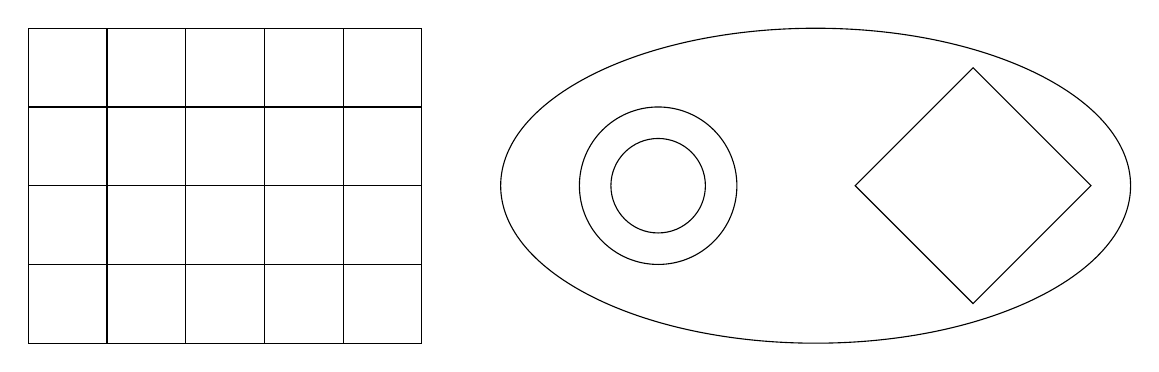
\begin{tikzpicture}[node distance=0cm]
\draw[step=1cm] (-5,-2) grid (0,2);

\draw(5,0) ellipse (4cm and 2cm);
\draw(3,0) circle (1cm);
\draw(3,0) circle (0.6cm);
\node [diamond,draw,minimum width=3cm,minimum height=3cm](d)  at (7,0){};
\end{tikzpicture}
\caption{دو تصویر}
\end{figure}
\end{document}